\documentclass[10pt,twocolumn,letterpaper]{article}

\usepackage{cvpr}
\usepackage{times}
\usepackage{epsfig}
\usepackage{graphicx}
\usepackage{cite}
\usepackage{amsmath}
\usepackage{amssymb}

% Include other packages here, before hyperref.

% If you comment hyperref and then uncomment it, you should delete
% egpaper.aux before re-running latex.  (Or just hit 'q' on the first latex
% run, let it finish, and you should be clear).
\usepackage[breaklinks=true,bookmarks=false]{hyperref}

\cvprfinalcopy % *** Uncomment this line for the final submission

\def\cvprPaperID{****} % *** Enter the CVPR Paper ID here
\def\httilde{\mbox{\tt\raisebox{-.5ex}{\symbol{126}}}}

% Pages are numbered in submission mode, and unnumbered in camera-ready
%\ifcvprfinal\pagestyle{empty}\fi
\setcounter{page}{2571}
\begin{document}

%%%%%%%%% TITLE
\title{	CNN Based Image Classification}

\author{Xiaoling Long\\
SIST\\
ShanghaiTech Univ.\\
{\tt\small longxl@shanghaitech.edu.cn}
% For a paper whose authors are all at the same institution,
% omit the following lines up until the closing ``}''.
% Additional authors and addresses can be added with ``\and'',
% just like the second author.
% To save space, use either the email address or home page, not both
\and
Hongyu Chen\\
SIST\\
ShanghaiTech Univ.\\
{\tt\small chenhy3@shanghaitech.edu.cn}
\and
Second Author\\
SIST\\
ShanghaiTech Univ.\\
{\tt\small secondauthor@i2.org}
}


\maketitle
%\thispagestyle{empty}

%%%%%%%%% ABSTRACT
\begin{abstract}
   The convolution networks make a great success in image classification since AlexNet proposed for classification in ImageNet chanllenge. This End-to-End training method make researcher focus more on how to build an efficient network. The user focus more on how to use convolution networks in their application. After AlexNet, there are many ConvNet architecture proposed, such as VGGNet  and ResNet. These ConvNet architectures are widely  used in many actual real applications.
\end{abstract}

%%%%%%%%% BODY TEXT
\section{Introduction}
Image classification is a fundamental challenge in computer vision\cite{felzenszwalb2013visual}. Consider the problem of detecting objects from a category, such as people or cars, in static images. This is a difficult problem because objects in each category can vary greatly in appearance. Variations arise from changes in illumination, viewpoint, and intra-class variability of shape and other visual properties among object instances. For example, people wear different clothes and take a variety of poses while cars come in various shapes and colors.Classification   between   the   objects   is   easy   task   for  humans  but  it  has  proved  to  be  a  complex  problem for machines.Image classification refers to the labeling of images into one of a number of predefined categories.
Image classification is an important and challenging task in various application domains, including biomedical imaging, biometry, video surveillance, vehicle navigation, industrial visual inspection, robot navigation, and remote sensing \cite{kamavisdar2013survey}.

Image classification uses both supervised and unsupervised
Traditional  methods  of  computer  vision  and  machine
learning cannot match human performance on tasks such
as the recognition of handwritten digits or traffic signs.\cite{ciregancolumn}

Non‐parametric  classifiers  such  as  decision tree   classifier,  neural   network,   SVM   classifier and knowledge based classification are also very common in image classification.

Disadvantages about the deep learning.For the deep learning based algorithm required the ability of labeled samples for training. The collection of labeled data is a time consuming process as well as costly.


%-------------------------------------------------------------------------
%\section{CNN Part}

\section{CNN Based Image classification}

\par
The ImageNet Large Scale Visual Recognition Challenge(ILSRC) is a benchmark in object category classification and detection on $1000$-classes and millions of images. After AlexNet achieved hugu success in ILSRC-2012, there are various variations of AlexNet\cite{krizhevsky2012imagenet} and many other types of ConvNet for image classification. Since that, ConvNet is widely used for image classification. \cite{aloysius2017review} illustrate beriefly what is ConvNet, the components of ConvNet, the activation function in ConvNet, from LeNet to ResNet bunch of successful ConvNet and some open issues on CNN based image classification. LeNet is first proposed CNN based image classifition method.

\par
LeNet\cite{lecun1990handwritten} is first proposed CNN based image classifition method. After that, AlexNet\cite{krizhevsky2012imagenet} brought Convolutional neural network into ILSRC. In this implementation, it contains 8 layers \- 5 convolutional and 3 fully-conneted. The main features of this network's architecture are ReLU\cite{nair2010rectified} as activation function, overlapping pooling and skills for reducing overfitting. Based on ReLU and overlapping pooling, the network err rate has more or less reduction, and ReLU network learn several times faster than other saturating acitvation function such as tanh neurons network. Overfitting is common issue for machine learning, it uses data augmentation and dropout to avoid overfit. Dropout is a skill to reduce argument or increase hypothesis. There are many discuss about this. As to data augmentation, it enlarge the dataset by cropping $224\times 224$ patched from the original image as well as these patchs' horizontal refliction. At the end averaging the predications as final socre.
\par
\cite{donahue2014decaf} explored the generalization ability of ConvNet features, releasing DeCAF. Traditional image classifition pipeline is extracting feature, building bag of feature then put into classifier. \cite{zeiler2011adaptive} propose a CNN based feature extractor. This is an unsurpervising learning ConvNet or in other words, input image is also the kind of ground truth. After feature extracting, the final result can classify by any classifier. This strategy is used as a tool for visualizing and undestanding how ConvNet works \cite{zeiler2014visualizing}.ConvNet have an impressive classification performance. However there is no clear understanding for why this work. \cite{zeiler2014visualizing} propose a architecture for visualizing and undestanding how ConvNet works.
\par
OverFeat\cite{sermanet2013overfeat} is a integrated recognition, localization and detection. This network uses CNN extract feature from image and then perform classification and localization and detection. Multi-scale classification brought up in \cite{sermanet2013overfeat} to increase accuracy.
\par
``Networ In Network"\cite{lin2013network} propsed a new deep network structure. Different from conventional convolution layer, it brings up a new Mlpconv layer. This Mlpconv layer consist of sliding multilayer perceptron(MLP) window. In stead of fully-connected layer at the top of network, global average pooling is used to produce the resulting vector fed directly into the softmax layer. Verified by experiments, this NIN structure indeed works well on some benchmark datasets, and global average pooling can be regarded as regularizer. THis glolbal average pooling has no parameter. This stratety is used widely afterwards. $1\times 1$ convolution conception proposed in \cite{lin2013network} is used in GoogLeNet for dimension reduction.

\par
AlexNet make a great success in image classification. Afterwards many various Network appear. GoogLeNet\cite{szegedy2015going} proposed by google is a new level of oganization in the form of the `` Inception module". This is a multi-scale arcthitecture. With the limitation of computational resource, it perform a $1\times 1 $ convolution to dimension reduction. Auxiliary classifier is also a brilliant strategy.This smart design makes a great success in ILSRC-2014. At the same time, the widely used ConvNet architecture VGGNet\cite{simonyan2014very}  won the first place in \textit{Classification $+$ Localization competition}. It adds the number of layers up to $16-19$. Instead of $7\times 7$ convolution filter in \cite{simonyan2014very}, it uses $3\times 3$ as convolution filter. After multiple layers, it can get similar effect as $7\times 7 $ one. This design significantly reduces the parameters, and then reduces the overfitting. It also means the number of layers significantly increases. Altering convolutional layers and poolint layer became a common used Network architecture.
\par
As the depth of ConvNet increasing, training gets more and more difficult. The training of very deep network becomes a open issue in CNN. Highway Networks\cite{srivastava2015highway, srivastava2015training} propose \textit{information highways} which allow unimpeded information flow across several layers. The \textit{transform gate} $T(x, W_{T})$ and the \textit{carry gate} $C(x, W_{C})$ proposed for decided how much flow pass through to output. The new model given by
\begin{equation}
  y_{output} = H(x, W_{H})\cdot T(x, W_{T}) + x\cdot C(x, W_{C})
\end{equation}
For simplicty, \cite{he2016deep} set $C = 1 - T$. This design make training hundreds of layers be possible and the err rate just has slightly increase. This architecture promote the success of ResNet \cite{he2016deep}. ResNet has similar structure as deep plain network stacked by dozens of convolution layers followed by global pooling layer and $1$ fully-connected layer. except shortcup connection. This design has a residual representation which called deep residual learning. This archicture keeps parameter less than VGG-19 model even the network has $152$ layers. This smart design make ResNet won first place in ILSRC-15.

There are several works based on region based image classification.Such as \cite{girshick2015fast},\cite{DSDFGVFB}\cite{uijlings2013selective},\cite{alexe2012measuring}. Region based methods are computationally expensively.


R-CNN and fast R-CNN is regioned based convolutional network method for object detection and image classification. In\cite{DSDFGVFB},they use the selective search to select those propose regions. Features are extracted from each proposal region. Then a SVM classifier is used for the category classification. This kind of algorithm need a  lot of time to process each image.  About $2000$ regions are proposed from each image where there maybe several objects in the image.


Compared to R-CNN\cite{DSDFGVFB}, Fast R-CNN\cite{girshick2015fast} employs several innovations to improve training and testing speed while also increasing detection accuracy. the fast R-CNN has several advantages: (1) higher detection quality  than  R-CNN ,(2) using  a multi task loss ,predict the object and its confidence. No disk storage is required for additional feature catching.The computation is shared during training. Fast achieves a near real time rates uses a very deep network.

Proposal based image classification also contains some great work. Such as \cite{ren2017faster}\cite{redmon2016you}\cite{Redmon2016YOLO9000}\cite{yolov3}.



Faster R-CNN\cite{ren2017faster} is another convolutional network which based on the region proposal methods. In \cite{ren2017faster},The author show that an algorithmic change computing proposals with a deep convolutional neural network leads to an elegant and effective solution where proposal computation is nearly cost-free given the detection network’s computation. They removed the select search algorithm replaced by a region proposal network.
The high quality proposal is used by the Fast R-CNN network for detection and classification. For the very deep VGG-16 model the detection system has a frame rate of 5fps (including all steps) on a GPU, while achieving state-of-the-art object detection accuracy.


Fast and Faster R-CNN focus on speeding up the R-CNN framework by sharing computation and using neural networks to propose regions instead
of Selective Search. While they offer speed and accuracy improvements over R-CNN, both still fall short of real-time performance.
Fast R-CNN speeds up the classification stage of R-CNN but it still relies on selective search which can take around 2 seconds per image to generate bounding box proposals.


In \cite{redmon2016you}, the author achieves a real time detection and classification in $45$  frames per second. A smaller version of their network can be achieved by $ 155$ frames per second. The problem is view as a regression task. The output of the net contains five parameters. $(x,y,w,h,confidence)$ where $x,y,w,h$ means x location , y  location, the width and the height of the target, the probabilistic of the cell contains an object respectively. YOLO shares some similarities with R-CNN. Each grid
cell proposes a potential bounding boxes and scores those boxes using convolutional features.

\cite{liu2016ssd},the author propose an algorithm which can runs real time object detect and classification. A key feature of the SSD algorithm is that multi-scale of the convolutional bounding boxes outputs are attached to different feature maps.SSD is faster than R-CNN and its variants.

\begin{figure}[htbp]
	\begin{center}
		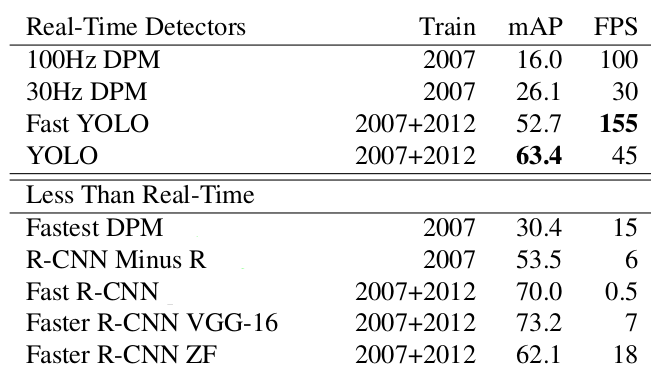
\includegraphics[width=0.8\linewidth]{./Pic/test.png}
	\end{center}
	\caption{Real-Time Systems on P ASCAL VOC 2007.Compar-
		ing the performance and speed of fast detectors. Fast YOLO is
		the fastest detector on record for P ASCAL VOC detection and is
		still twice as accurate as any other real-time detector. YOLO is
		10 mAP more accurate than the fast version while still well above
		real-time in speed.}
	\label{fig:lxsfvgong}

	Figure\ref{fig:lxsfvgong} shows the most famous network on image classification. The accuracy and the speed is shown on the table.

\end{figure}

\section{CNN based Medical Image Classification}

%-------------------------------------------------------------------------
\subsection{Introduction}

Convolutional neural networks (CNNs) have been used in the field of computer vision for decades. However, their true value had not been discovered until the ImageNet competition in 2012, a success that brought about a revolution through the efficient use of graphics processing units (GPUs), rectified linear units, new dropout regularization, and effective data augmentation. Acknowledged as one of the top 10 breakthroughs of 2013, CNNs have once again become a popular learning machine, now not only within the computer vision community but across various applications ranging from natural language processing to hyperspectral image processing and to medical image analysis. The main power of a CNN lies in its deep architecture, which allows for extracting a set of discriminating features at multiple levels of abstraction\cite{tajbakhsh2016convolutional}.

However, training a deep CNN with full training is very complicated. First, CNNs require a large
amount of labeled training data. Second, training a deep CNN requires extensive computational and memory resources, without that the training process would be extremely time-consuming.Third, training a deep CNN is often complicated by overfitting. Therefore, deep learning from scratch can be tedious and time-consuming, demanding a great deal of diligence, patience, and expertise.

In this survey, I conducted an extensive set of experiments for 4 medical imaging applications: 1) polyp detection in colonoscopy videos~\cite{ribeiro2016colonic}\cite{zhang2017automatic}, 2) image quality assessment and classification in tissues and cells such as blood vessels videos\cite{mcilroy2017vivo}\cite{li2017cell}\cite{huang2017epithelium}\cite{kieffer2017convolutional}\cite{hadad2017classification}\cite{araujo2017classification}, 3) lung disease such as pulmonary embolism detection and so on in computed tomography (CT) images\cite{shen2015multi}\cite{li2014medical},4) dental disease in X-ray image\cite{prajapaticlassification} and 5) intima-media boundary segmentation in ultrasonographic images\cite{roth2015anatomy}.

\subsection{Polyp Detection}

Colorectal cancer (CRC) is one of the leading causes of deathworldwide with about estimated 700 thousand deaths in 2012\cite{zhang2017automatic}. Long-term follow-up studies confirmed that removal of adenomatous polyps reduces CRC mortality. Colonoscopy is the preferred technique for colon cancer screening and prevention. The goal of colonoscopy is to find and remove colonic polyps—precursors to colon cancer. But polyps can appear with substantial variations in color, shape, and size. The challenging appearance of polyps can often lead to misdetection\cite{ribeiro2016colonic}. Polyp miss-rates are estimated to be about 4\% to 12\%; however, a more recent clinical study is suggestive that this misdetection rate may be as high as 25\%. So nowadays, there are many research groups start to use computer aided method such as CNN.

In the article\cite{ribeiro2016colonic}, the author have a small dataset, which only have 100 images(75 abnormal images and 25 healthy images). After finishing the data augmentation which results in 800 images, they resized the 256*256 image to 128*128. In order to test the five architecture they established, he used cross validation method(56 for training and 6 for testing), the result can be seen in Figure 1, the accuracy is just 75\% to 80\%.

\begin{figure}[t]
	\begin{center}
		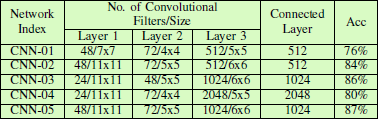
\includegraphics[width=0.8\linewidth]{Pic/4.png}
	\end{center}
	\caption{Accuracy results from different CNN configurations}
	\label{fig:long}
	\label{fig:onecol}
\end{figure}

In order to improve the accuracy, in the evaluation phase, the author obtained the final decision for a 256*256 pixel image by majority voting of the decisions of all 128*128 pixel subimages(patches). This is a kind of fine-tuning. The redundancy of overlapping subimages can increase the system accuracy likewise to give the assurance of certainty for the overall decision. The result can be seen in figure 2. They also perform a random patch extraction and it can be concluded that there is not much difference between 16384 subimages or
just 32 subimages (accuracy of 90.96\%), saving considerable computation time and achieving good results.

\begin{figure}[t]
	\begin{center}
		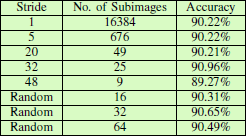
\includegraphics[width=0.8\linewidth]{Pic/5.png}
	\end{center}
	\caption{Accuracy of different strides for overlapping subimages in the evaluation.}
	\label{fig:long}
	\label{fig:onecol}
\end{figure}

In the second article\cite{zhang2017automatic}, the author use a small datasets(PHW Database), this dataset consisted of 1104, 263 and
563 images without polyps, with hyperplasia polyps and adenomatous polyps, respectively, taken under either WL or NBI endoscopy. For fair comparison, 50 images from each class (nonpolyp, hyperplasia, and adenoma) were randomly selected as testing dataset, while the rest were treated as training dataset.

Because this dataset has an imbalanced number of images for each class, Previous study for polyp detection proposed to use an up/down sampling strategy to tackle such challenge. In this paper, the authors randomly down sampled the majority class to match the sample size of the minority class for both target tasks. The source dataset used ILSVRC and Places205 and trained for 450 000 iterations. They tested two tasks using this database, first is polyp detection and second polyp type classification. In order to do the evaluation, the authors used a feature engineering technique: bag-of-words for comparison. After finishing these tasks, we can see the results in the Figure 3.4.5. In these figures, we can see that transferring low-level CNN features gives better transfer learning performance for both target tasks and when a CNN structure is directly
used for detection and classification. The performance of the proposed method is better in both tasks.

\begin{figure}[t]
	\begin{center}
		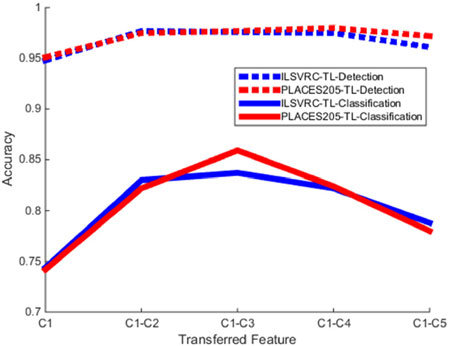
\includegraphics[width=0.8\linewidth]{Pic/6.jpg}
	\end{center}
	\caption{Average accuracy of the detection and classification tasks by transferring C1–Cn features learned from ILSVRC and Places205 and using SVM as the classifier with a RBF kernel.}
	\label{fig:long}
	\label{fig:onecol}
\end{figure}

\begin{figure}[t]
	\begin{center}
		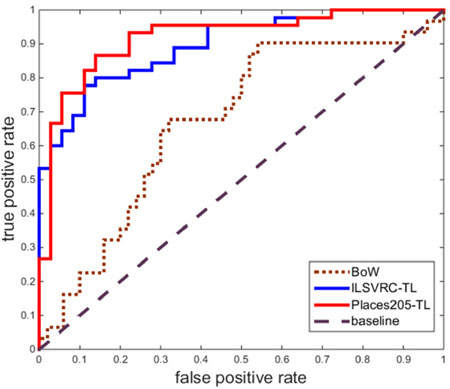
\includegraphics[width=0.8\linewidth]{Pic/7.jpg}
	\end{center}
	\caption{Typical ROC curve for polyp classification for PWH database.}
	\label{fig:long}
	\label{fig:onecol}
\end{figure}

\begin{figure}[t]
	\begin{center}
		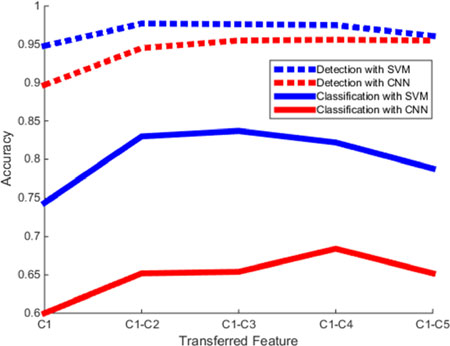
\includegraphics[width=0.8\linewidth]{Pic/8.jpg}
	\end{center}
	\caption{Average accuracy of the detection and classification tasks by transferring C1–Cn features learned from ILSVRC and using either RBF kernel SVM or a fully connected CNN layer with a softmax classifier}
	\label{fig:long}
	\label{fig:onecol}
\end{figure}

\subsection{Tissue Detection and Classification}

In this part, I will choose two typical article to discuss. In the first article\cite{kieffer2017convolutional}, the author used feature vectors from several pre-trained structures, including networks with/without transfer learning to evaluate the performance of pre-trained deep features versus CNNs which have been trained by that specific dataset as well as the impact of transfer learning with a small number of samples. This experiment is done on Kimia Path24 dataset which consists of 27,055 histopathology training patches in 24 tissue texture classes along with 1,325 test patches for evaluation. In order to do this experiment, the author used fine-tuning method and a pre-trained CNN as a feature extractor and a fine-tuned CNN as a classifier.

\begin{figure}[t]
	\begin{center}
		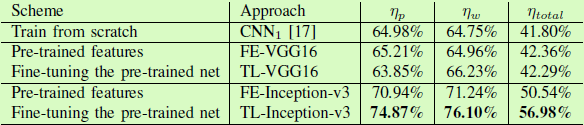
\includegraphics[width=0.8\linewidth]{Pic/12.png}
	\end{center}
	\caption{Comparing the results training form scratch , using deep features via a pre-trained network with no change (FE-VGG16), and classification after fine-tuning a pre-trained network (TL-VGG16, TL-Inception-v3). The best scores are highlighted in bold.(\textit{$\eta_p$} means the patch-to-scan accuracy and \textit{$\eta_n$} means whole-scan accuracy)}
	\label{fig:long}
	\label{fig:onecol}
\end{figure}

The result shows in figure 6 that pre-trained networks are quite competitive against training from scratch. In this figure, VGG16 and CNN are quite similar, whereas the results for Inception-v3 are similar with the transfer-learned model outperforming the feature extractor. But considering Inception-v3 requires no extra effort and produces similar results with a linear SVM, one may prefer using it to training from scratch and fine-tuning a pre-trained net.

In the next article\cite{araujo2017classification}, the authors designed a specific CNN network which perform image-wise classification in four classes of medical relevance: normal tissue, benign lesion, in situ carcinoma and invasive carcinoma. The proposed CNN architecture is designed to integrate information from multiple histological scales, including nuclei, nuclei organization and overall structure organization. A data augmentation method is adopted to increase the number of cases in this training set. A SVM classification using the features extracted by the CNN is also used for comparison purposes.

The dataset is composed of an extended training set of 249 images, and a separate test set of 20 images. In these datasets, the four classes are balanced. The images were selected so that the pathology classification can be objectively determined from the image contents. An additional
test set of 16 images is provided with images of increased ambiguity, which they denote as extended dataset.

They first normalized the images. First, the colors of the images are converted to optical density (OD) using a logarithmic transformation. Then, they used singular value decomposition (SVD)  to the OD tuples to find the 2D projections with higher variance. The resulting color space transform is then applied to the original image. Finally, the image histogram is stretched so that the dynamic range covers the lower 90\% of the data.

Then they do two kinds of classification: Image-wise classification and CNN patch-wise classification. Image-wise classification first divided the origin image into twelve contiguous non-overlapping patches and then use one of three different patch patch methods: majority voting, maximum probability and sum of probabilities. CNN patch-wise classification used 75\% of the data to do the training and validated on the remaining images.The validation set is randomly selected for each epoch. The training process stops after the stabilization of the validation accuracy with equal weight for all the classes (50 epochs). The authors also used the features extracted by the CNN to train a SVM classifier to do the comparison. The result can be seen in figure 7, 8 and 9.

\begin{figure}[t]
	\begin{center}
		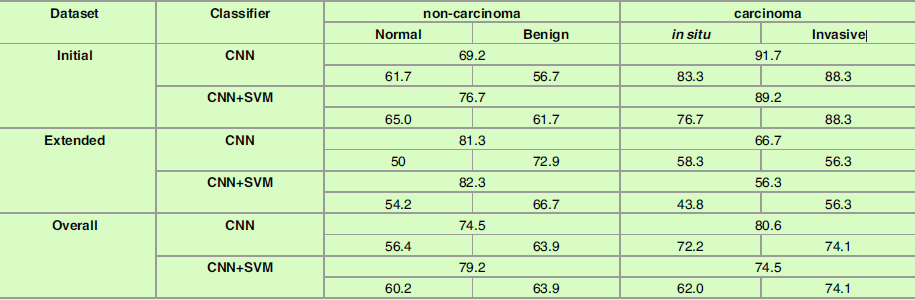
\includegraphics[width=0.8\linewidth]{Pic/13.png}
	\end{center}
	\caption{Patch-wise sensitivity (\%) (2 and 4 classes).}
	\label{fig:long}
	\label{fig:onecol}
\end{figure}

\begin{figure}[t]
	\begin{center}
		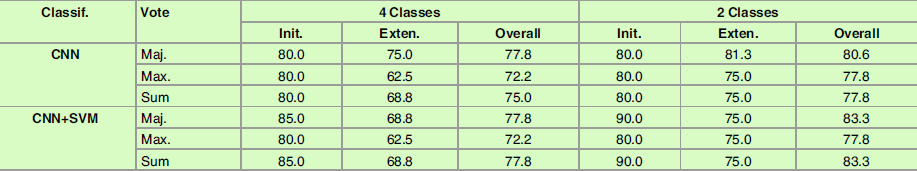
\includegraphics[width=0.8\linewidth]{Pic/15.png}
	\end{center}
	\caption{Image-wise accuracy (\%) using different voting rules (2 and 4 classes).}
	\label{fig:long}
	\label{fig:onecol}
\end{figure}

\begin{figure}[t]
	\begin{center}
		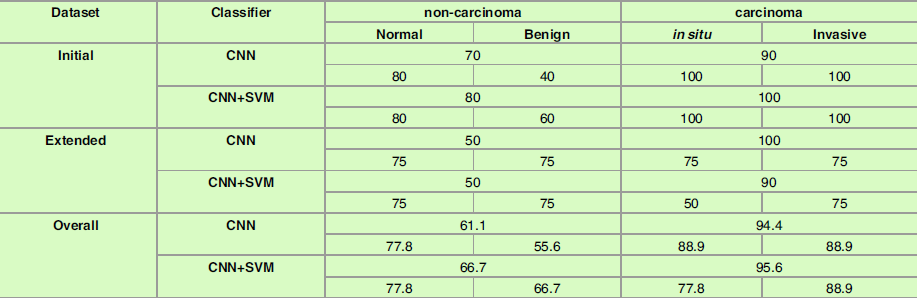
\includegraphics[width=0.8\linewidth]{Pic/14.png}
	\end{center}
	\caption{Image-wise sensitivity (\%) using majority voting (2 and 4 classes).}
	\label{fig:long}
	\label{fig:onecol}
\end{figure}

In figure 7, we can see the result similar between the CNN and CNN+SVM. But the performance of this network is lower for the extended dataset due to its increased complexity. In figure 8 and 9, we can see that CNN+SVM get the best result with the majority voting method. In comparison, CNN's performance is only better for the extended set using majority voting. In addition, we can see that maximum probability is the worst performing method in both methods, which means that this method is not suit in this case.

\subsection{Some kinds of lung Diseases Classification}

Lung cancer is notoriously aggressive with a low long-term survival rate. Quantitative analysis in lung nodules using thoracic Computed Tomography(CT) has been a central focus for early cancer diagnosis, where CT phenotype provides a powerful tool to comprehensively capture nodule characteristics. The importance of diagnostically classifying malignant and benign nodules using CT images is to facilitate radiologists for nodule staging assessment and individual therapeutic planning.\cite{shen2015multi}

In the first article\cite{shen2015multi}, the authors used the LIDC-IDRI datasets, which has 1375 nodule pictures(1100 for training and 275 for testing). In order to improve the speed and accuracy, the authors introduced an Multi-scale Convolutional Neural Networks(MCNN) model to do the lung nodule diagnostic classification. This CNN model take multi-scale raw nodule patches and remove the need of any hand-crafted feature engineering work. This network can also deal with noisy data in nodule CT.

Because of the clinical fact that nodule sizes vary remarkably, this network take patches from different scales(3 layers) as inputs in parallel. The parameter is shared between these layers to reduce parameter. When doing the evaluation task, the result is decided by all the layers. The authors use the HOG and uniform LBP descriptor and SVM and RF classifier to do the classification. The result can be seen in figure 6 and figure 7. In figure 7, the \textit{$S_w$} means the size of the cell window for SVM and \textit{$n_{pt}$} means the number of neighbourhood points for LBP.

\begin{figure}[t]
	\begin{center}
		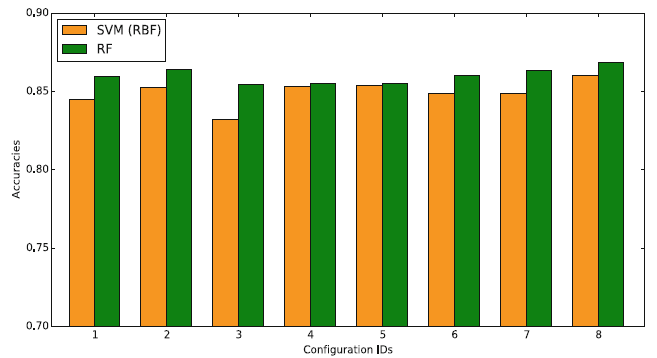
\includegraphics[width=0.8\linewidth]{Pic/9.png}
	\end{center}
	\caption{The classification performance of SVM with the RBF kernel and RF based on features from the MCNN using 8 different configurations. Each configuration is assigned to a unique ID for display convenience}
	\label{fig:long}
	\label{fig:onecol}
\end{figure}

\begin{figure}[t]
	\begin{center}
		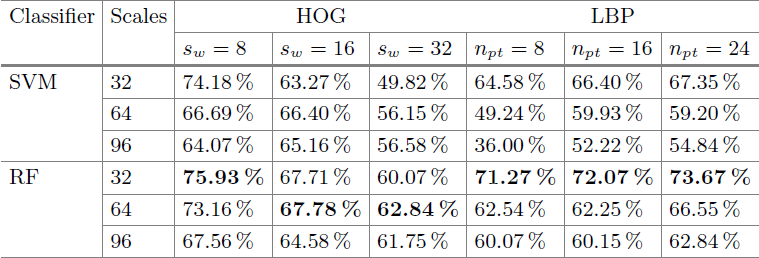
\includegraphics[width=0.8\linewidth]{Pic/10.png}
	\end{center}
	\caption{Performance using the HOG and LBP descriptors with different \textit{$S_w$} and \textit{$n_{pt}$}}
	\label{fig:long}
	\label{fig:onecol}
\end{figure}

The second article\cite{li2014medical} is about using CNN to classify the ILD patterns. This experiment used an ILD database which contains 113 sets of HRCT images, with 2062 2D regions indicting the ILD category. In order to augment the dataset, the CT slices were divided into half-overlapping image and the only if 75\% percent of its pixels falling inside the regions of interest will be adopted. The dataset thus contains 16220 image patches from 92 HRCT image sets,
including 4348 norm patches, 1047 emphysema patches, 1953 ground glass patches, 2591 fibrosis patches, and 6281 micronodules patches.

The authors compared their classification results with three other feature extraction approaches: SIFT feature, LBP feature and unsupervised feature learning using RBM. The result can be seen in Figure 8. In this figure, we can see that their customized CNN method achieved the best classification preformance.

\begin{figure}[t]
	\begin{center}
		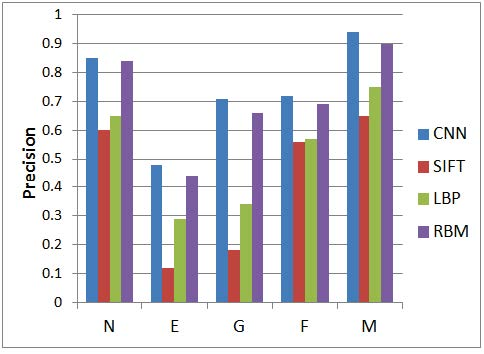
\includegraphics[width=0.8\linewidth]{Pic/11.jpg}
	\end{center}
	\caption{The classification results comparing proposed customized CNN method with SIFT, LBP and RBM}
	\label{fig:long}
	\label{fig:onecol}
\end{figure}

\subsection{Dental Disease Classification in X-ray Images}

The author found that there is no literature for dental disease classification, so the research group start to use CNN to deal with X-ray images and make some breakthrough. Orthopantomogram (OPG) and Radiovisiography (RVG) x-ray images are the most widely used tools for the diagnoses of dental diseases. Dental caries is one of the most common dental disease worldwide and it has different stages. So the CNN network in this experiment is used to classify mainly 3 classes (dental caries, periapical infection, periodontitis)\cite{prajapaticlassification}.

Because though the radiologists have large dataset of dental x-ray images, these x-ray images have individual privacy issues. So the dataset is very small in this experiment, just have 251 grey images of dimension 1000*1496. So the authors use transfer learning method to do the fine tuning and improve the accuracy very much. They changed some unfrozen layers used for training in order for the pre-trained model to be more adaptive to the training data.

They first resize these picture to 500*748, and then use 180 of 251 to do the training, 45 images for validation and 26 images for testing purpose. Because of the unavailability of the large dataset, CNN architecture could not perform well in this classification task. After they used transfer learning model to do the fine tuning, the accuracy is increased by 15.39\% compared to pure CNN model, and achieved 88.46\% accuracy, which is very encouraging.

\begin{figure}[t]
	\begin{center}
		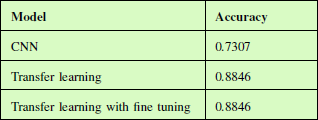
\includegraphics[width=0.8\linewidth]{Pic/2.png}
	\end{center}
	\caption{The comparison of different models}
	\label{fig:long}
	\label{fig:onecol}
\end{figure}

\begin{figure}[t]
	\begin{center}
		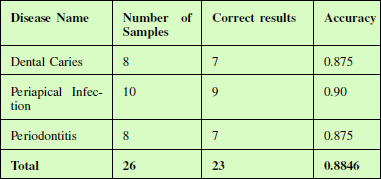
\includegraphics[width=0.8\linewidth]{Pic/3.png}
	\end{center}
	\caption{Experimental results for transfer learning model}
	\label{fig:long}
	\label{fig:onecol}
\end{figure}

\subsection{Intima-media Boundary Segmentation}

Automated classification of human anatomy is an important prerequisite for many computer-aided diagnosis systems. The spatial complexity and variability of anatomy throughout the human body makes classification difficult. So the authors want to use CNN to do this classification. In this paper, the authors choose to use 4298 separate axial 2D key images to learn 5 anatomical classes(neck, lungs, liver, pelvis and legs)\cite{roth2015anatomy}.

When applying the CNN to build the anatomy-specific classifier for CT images, because the authors want to classify these picture to 5 classes, so they choose 5 cascaded layers. All the convolutional filter kernel elements are trained from the data in a supervised fashion. In order to avoid overfitting, the fully-connected layers are constrained, using the \textit{DropOut} method. The datasets are from the Picture Archiving and Communication System (PACS) of the Clinical Center of the National Institutes of Health. In order to enrich their data, they use spatial deformations to each image, using random translation, rotations and non-rigid deformations, which lead their datasets from hundred's picture to near 100 thousand pictures. Before import into the CNN, the author resize all the picture to 256*256 pixels.The authors use 80\% of their total dataset to train the CNN and reserve 20\% to do the test. After doing the experiments, the accuracy of this net can reach 94.1\%, which can be seen in figure 4.This classification
result is achieved in less than 1 minute on a modern desktop computer and GPU card (Dell Precision T7500,
24GB RAM, NVIDIA Titan Z).

\begin{figure}[t]
	\begin{center}
		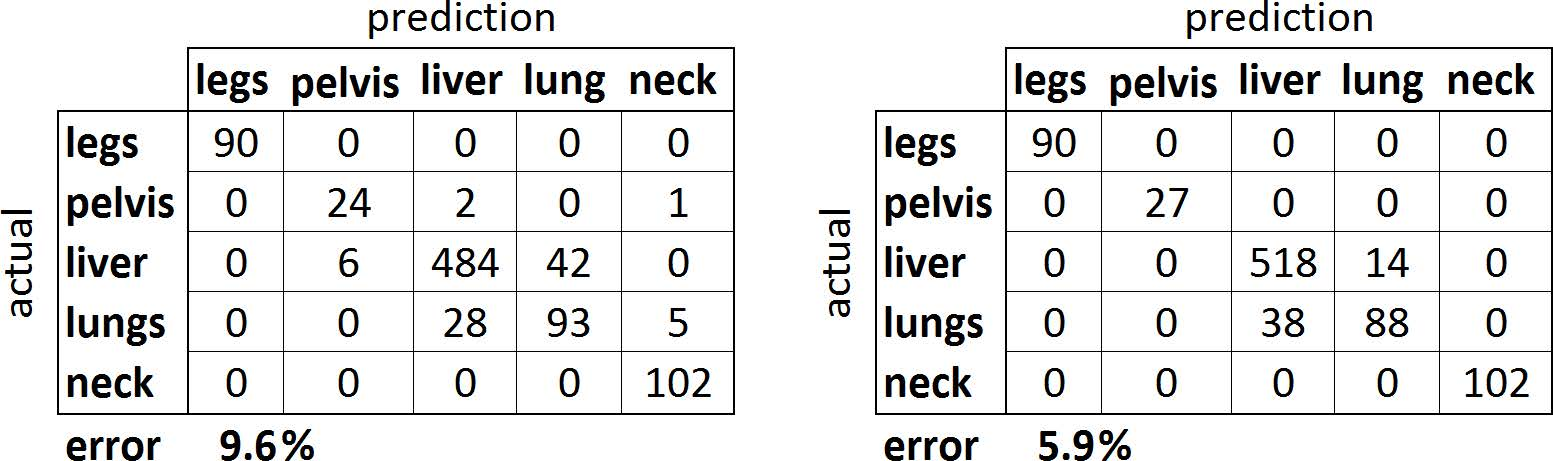
\includegraphics[width=0.8\linewidth]{Pic/1.jpg}
	\end{center}
	\caption{Confusion matrices on the original test images before and after data augmentation.} \label{fig:long}
	\label{fig:onecol}
\end{figure}

\subsection{Conclusion}

In this part, I aimed to address to know how the CNN can be used on the medical image classification and the result these experiments made. My experiment, based on 4 distinct medical imaging applications from different imaging modality systems, have demonstrated that deep CNN are useful for medical image analysis. If the training data is limited, the fine-tuned CNN can perform better than fully trained CNN. I think the potential of CNNs for medical imaging applications is confirmed because both deeply fine-tuned CNNs and fully trained CNNs can outperform the corresponding handcrafted alternatives. We can also see that the speed is depend on the devices, the more powerful the graphics is, the quicker the CNN network use to train.
%\section{Application}

\section{Conclusion}

In this paper we have discussed about the different types of image classification techniques and many CNN based medical application. So this paper will help us in selecting an appropriate classification technique among all the available techniques.


\newpage
{\small
\bibliographystyle{ieee}
\bibliography{egbib}
}

\end{document}
